\documentclass[border=6pt]{standalone}
\usepackage{tikz}
\usetikzlibrary{positioning,arrows.meta,fit,backgrounds,shapes.geometric}
\definecolor{navy}{HTML}{161E29}
\definecolor{slate}{HTML}{2E3D50}
\definecolor{slatefill}{HTML}{E9EDF2}
\definecolor{accent}{HTML}{B45309}
\definecolor{accentfill}{HTML}{FEF3C7}
\definecolor{edge}{HTML}{51647D}
\begin{document}
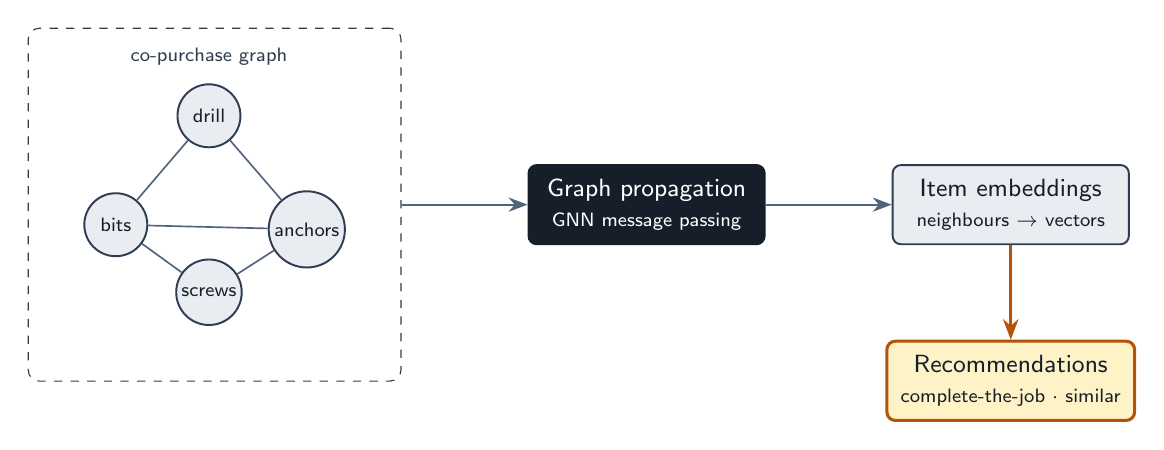
\begin{tikzpicture}[
  font=\sffamily\small,
  box/.style={rounded corners=3pt, draw=slate, line width=0.7pt, fill=slatefill, text=navy, align=center, inner sep=5pt, minimum height=10mm, minimum width=30mm},
  dark/.style={box, fill=navy, draw=navy, text=white},
  acc/.style={box, draw=accent, line width=1.1pt, fill=accentfill, text=navy},
  prod/.style={circle, draw=slate, line width=0.7pt, fill=slatefill, text=navy, inner sep=1.5pt, minimum size=8mm, font=\sffamily\scriptsize},
  lbl/.style={font=\sffamily\scriptsize, text=slate},
  arr/.style={-{Stealth[length=2.4mm]}, line width=0.8pt, draw=edge},
  accarr/.style={-{Stealth[length=2.6mm]}, line width=1.1pt, draw=accent},
  coedge/.style={draw=edge, line width=0.6pt},
]
\node[prod] (p1) {drill};
\node[prod, below left=8mm and 6mm of p1] (p2) {bits};
\node[prod, below right=8mm and 6mm of p1] (p3) {anchors};
\node[prod, below=14mm of p1] (p4) {screws};
\draw[coedge] (p1)--(p2);
\draw[coedge] (p1)--(p3);
\draw[coedge] (p2)--(p4);
\draw[coedge] (p3)--(p4);
\draw[coedge] (p2)--(p3);
\node[lbl, above=1mm of p1] {co-purchase graph};
\begin{scope}[on background layer]
\node[draw=slate, dashed, rounded corners=4pt, fit=(p1)(p2)(p3)(p4), inner sep=7mm] (graph) {};
\end{scope}
\node[dark, right=16mm of graph] (gnn) {Graph propagation\\{\scriptsize GNN message passing}};
\node[box, right=16mm of gnn] (emb) {Item embeddings\\{\scriptsize neighbours $\to$ vectors}};
\node[acc, below=12mm of emb] (rec) {Recommendations\\{\scriptsize complete-the-job $\cdot$ similar}};
\draw[arr] (graph) -- (gnn);
\draw[arr] (gnn) -- (emb);
\draw[accarr] (emb) -- (rec);
\end{tikzpicture}
\end{document}
